\documentclass{article}
\usepackage[utf8]{inputenc}
\usepackage{graphicx}
\usepackage[a4paper, left=1in, right=1in, top=1in, bottom=1in]{geometry}

\title{Network of Favors in P2P cloud federation}
\author{Gustavo Diniz Monteiro \\ \href{gustavo.monteiro@ccc.ufcg.edu.br, gustavo.d.monteiro@icloud.com} }
\date{December 2018}

\begin{document}

\maketitle

\section{Modality}

This work will follow the project portfolio modality and aims to implement a previously described concept of Network of Favors\cite{nof}, focusing on aspects of software engineering and the platform usability.

\paragraph{Mentor:} Francisco Vilar Brasileiro

\section{Abstract}
Many organizations have extreme fluctuations of use, and during these peaks, they have to resort to public clouds to meet fleeting demand. The cost of such an action in itself can be expensive, which together with possible sub-utilization of the resources belonging to the organization can generates high costs. The objective of this work is to present a way of implantation and incentive justice on resources sharing in P2P systems, initially using the direct reciprocity model called Network of Favors. The model that will be used for small and medium-sized networks, for scenarios where repeated peer interaction is most likely and where these organizations could meet their demand at peak times and offer favors in under utilization, with guarantee of protection against uncooperative members. In addition, the network focuses on being a lightweight solution and designed to be a pluggable and adaptable element to the provider, using first-hand knowledge gained by each member through direct interaction with other peers.

\section{The Problem}
Organizations with varying demand patterns and utilization peaks often resort to public clouds (cf. “cloud bursting”\cite{cloudburst}) to meet unexpected or short-term needs, thus escaping failures in meeting business demands and quality of service goals.
However, outside of peak times, the resources belonging to these organizations may become inactive, which is a loss of efficiency.

Under these circumstances, selling these surplus resources may be an interesting option for large private cloud providers, but not for smaller private providers.

One alternative that small and medium-sized private cloud providers may find advantageous is to collaboratively exchange idle capacity on a peer-to-peer (P2P) basis within a federation. In this case, each provider in the federation acts both as a resource provider (outside peak hours) and as a resource consumer (during peak times). In particular private cloud providers, because of the usually limited amount of own resources, would benefit greatly from this exchange\cite{fairness-benefices}, thus allowing them to access a larger pool of resources when local demand is too high and can not be met using only local resources and resources that simply do not exist locally.

\section{Objectives}
The objective of this work is the implementation of a system of network deployment of favors that allows the sharing of resources in P2P networks, functioning as a guarantor of justice and connectable to the federation provider.

Working as a middleware for favors requests, and defining functional interfaces that allow support to different providers of federations and justice algorithms for Network of Favors through specific modules for each provider and chosen justice algorithm that implement these interfaces, which will act as adapters, aiming to be a platform configurable and adaptable to the model of justice and to the provider of the federation of those who propose to use it.

\begin{figure}[h!]
    \centering
    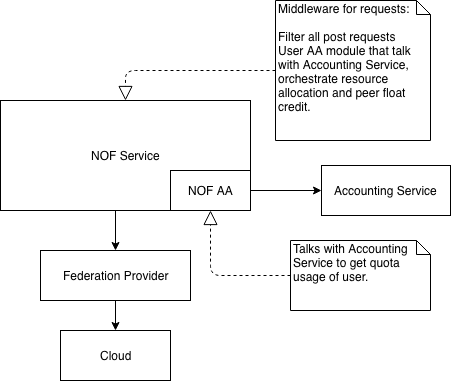
\includegraphics[scale=0.4]{./image/NOF-architecture-generic.png}
    \caption{NOF Architecture}
\end{figure}

During this work the default modules of connection with the federation provider, which will be the Fogbow (www.fogbowcloud.org), and the simple direct reciprocity justice algorithm will also be developed.

\section{Activities and Schedule}

\subsection{Activities}
The development of this study is planned to take place between January and June of the referent year of 2019 and will be divided into 3 main stages:

\begin{itemize}
    \item Development of application business logic: 
	Will be developed the interfaces and the default implementation of the components of the NOF service, in addition to constructing the flows the allocation of requisitions and the quota re-sizer.
	\item Development of integration tests:
	Will be developed the integration tests of the NOF components with default modules to test all of the most common streams of resource requests, non-cooperative member detection and the platform resiliency.
	\item Write the paper:
	Dedicated to the writing of the article, where all the decisions of software engineering and re results obtained with the NOF tool will be discussed for this work, which includes all the revisions of the article and possible revisions of architecture and/or implementation in the NOF.
\end{itemize}
    
\subsection{Schedule}
\begin{figure}[h!]
    \centering
    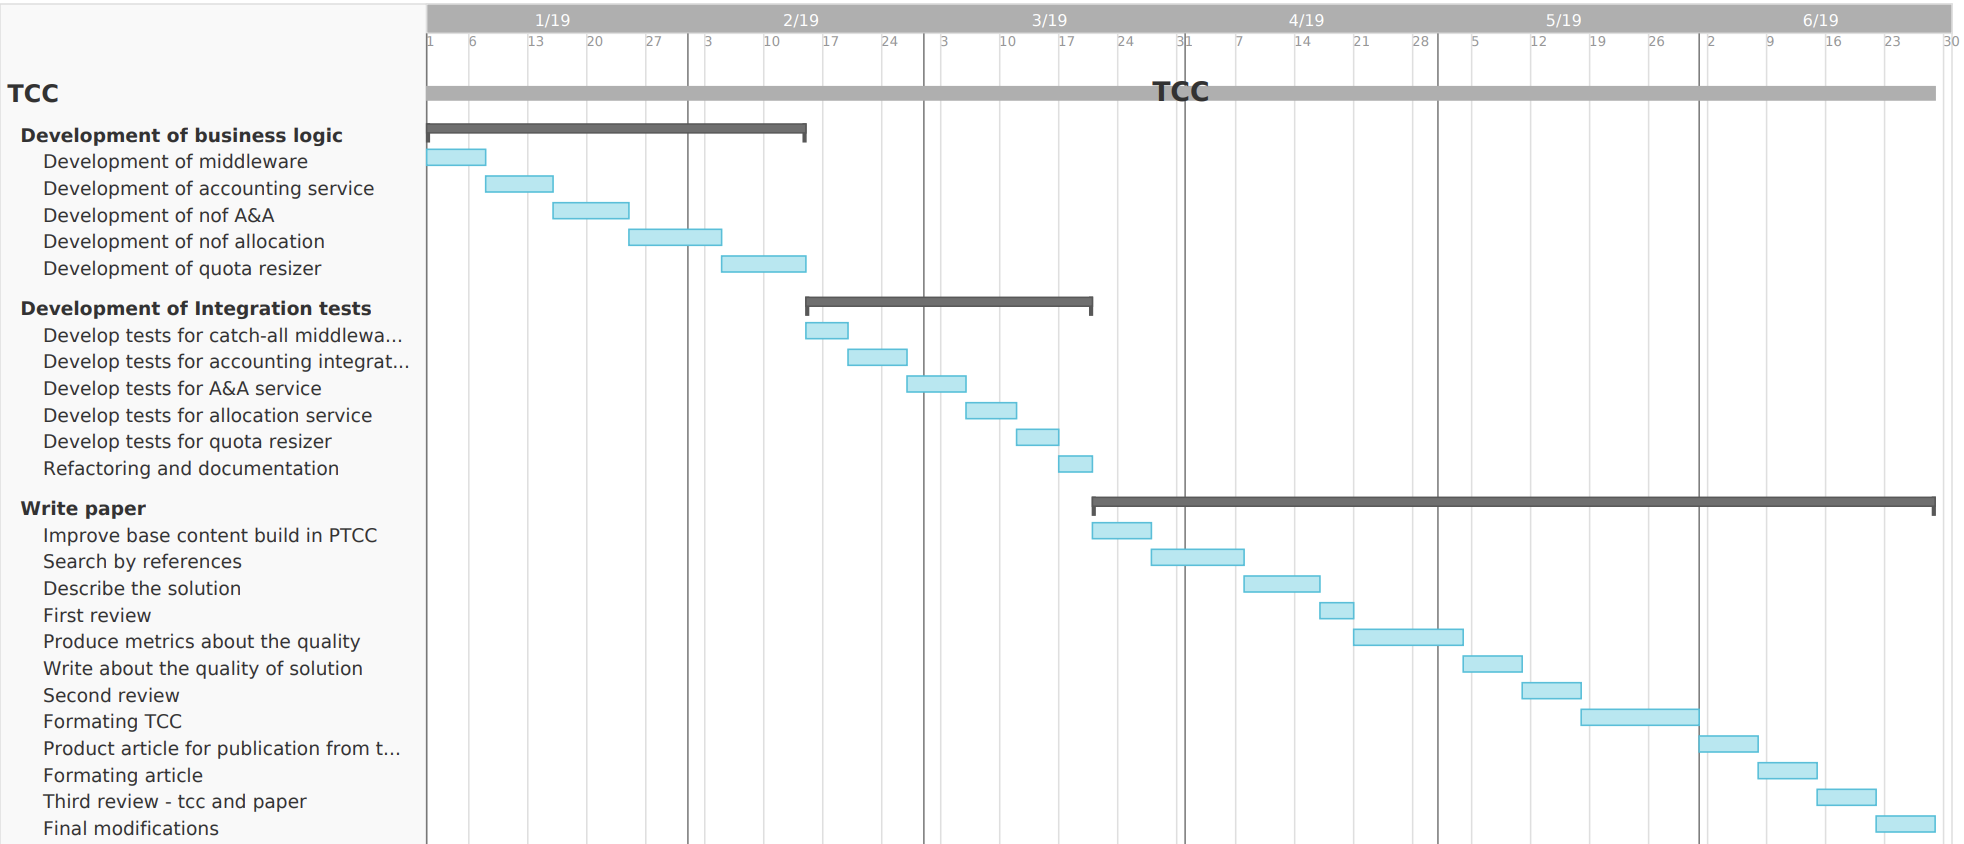
\includegraphics[scale=0.35]{./image/TCC-schedule.png}
    \caption{Activities Schedule}
\end{figure}

\begin{thebibliography}{9}

\bibitem{nof} 
N. Andrade, F. Brasileiro, W. Cirne, and M. Mowbray, “Automatic grid
assembly by promoting collaboration in peer-to-peer grids,” Journal of
Parallel and Distributed Computing, vol. 67, no. 8, pp. 957 – 966, 2007.

\bibitem{cloudburst}
Marshall P, Keahey K, Freeman T. Elastic site: using clouds to elastically extend site resources. In: Conference on cluster, cloud, and grid computing
(CCGRID); 2010. p. 43–52.

\bibitem{fairness-benefices}
Gomes ER, Vo QB, Kowalczyk R. Pure exchange markets for resource sharing in federated clouds. Concurrency Comput 2012;24(9):977–91.
\end{thebibliography}
    
\end{document}